\documentclass[border=10pt]{standalone}

\usepackage{tikz}
\usepackage{tikzsymbols}
\usetikzlibrary{calc,patterns,shapes.geometric}

\def\centerarc[#1](#2)(#3:#4:#5){\draw[#1] ($(#2)+({#5*cos(#3)},{#5*sin(#3)})$) arc (#3:#4:#5);}

\begin{document}
	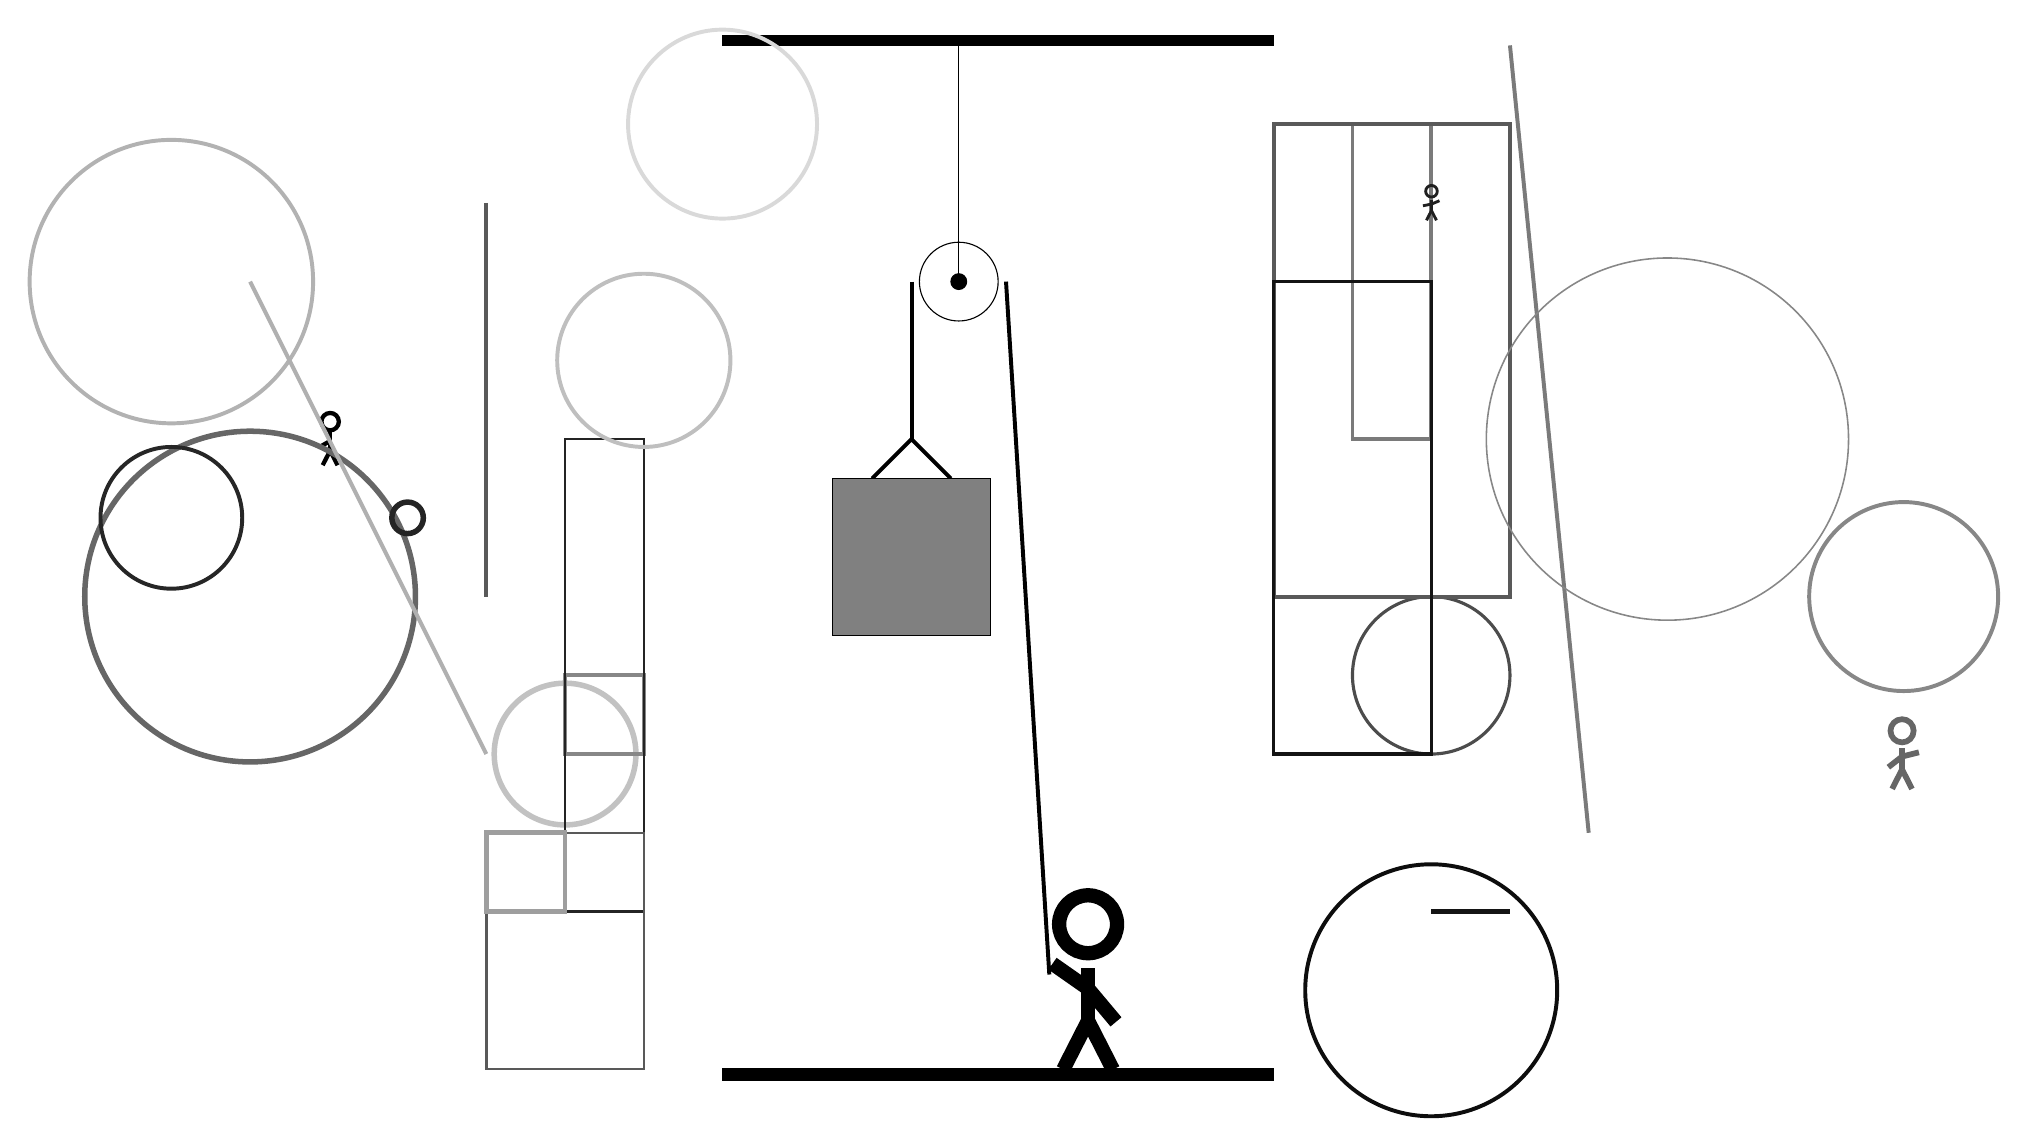
\begin{tikzpicture}
		%%%%% START %%%%%
		
		\draw[fill=black] (-2, 10) rectangle (5, 10.125);
		
		\draw (1, 7) circle (0.5);
		\draw[fill=black] (1, 7) circle (0.1);
		\draw (1, 10) -- (1, 7);
		
		\draw[line width=0.5mm] (-0.1, 4.5) -- (0.4, 5.0) -- (0.9, 4.5);
		\draw[fill=black!50] (-0.6, 4.5) rectangle (1.4, 2.5);
		
		\draw[line width=0.5mm, color=black!52] (7, 5) rectangle (6, 9);
		
		\node[line width=0.7mm, color=black!100] at (-7, 5) {\Strichmaxerl[3][30][90]};
		\draw [line width=0.4mm, color=black!70](7, 2) circle (1.0);
		\draw[line width=0.5mm, color=black!65] (5, 3) rectangle (8, 9);
		\draw [line width=0.7mm, color=black!24](-4, 1) circle (0.9);
		\node[line width=0.2mm, color=black!88] at (7, 8) {\Strichmaxerl[2][11][23]};
		\node[line width=0.6mm, color=black!60] at (13, 1) {\Strichmaxerl[4][38][14]};
		\draw[line width=0.4mm, color=black!92] (7, 7) rectangle (5, 1);
		\draw[line width=0.5mm, color=black!47] (-4, 2) rectangle (-3, 1);
		\draw[line width=0.3mm, color=black!86] (-3, 5) rectangle (-4, -1);
		
		\draw[line width=0.5mm, color=black!52](9, 0) -- (8, 10);
		\draw [line width=0.5mm, color=black!25](-3, 6) circle (1.1);
		\draw [line width=0.7mm, color=black!60](-8, 3) circle (2.1);
		
		\draw [line width=0.2mm, color=black!47](10, 5) circle (2.3);
		\draw [line width=0.5mm, color=black!15](-2, 9) circle (1.2);
		\draw [line width=0.5mm, color=black!30](-9, 7) circle (1.8);
		\draw [line width=0.5mm, color=black!47](13, 3) circle (1.2);
		\draw [line width=0.5mm, color=black!95](7, -2) circle (1.6);
		\draw[line width=0.5mm, color=black!31](-5, 1) -- (-8, 7);
		
		\draw [line width=0.5mm, color=black!85](-9, 4) circle (0.9);
		\draw [line width=0.7mm, color=black!86](-6, 4) circle (0.2);
		
		\draw[line width=0.5mm, color=black!65](-5, 8) -- (-5, 3);
		\draw[line width=0.7mm, color=black!92] (7, -1) rectangle (8, -1);
		\draw[line width=0.3mm, color=black!65] (-3, -3) rectangle (-5, 0);
		\draw[line width=0.6mm, color=black!38] (-4, 0) rectangle (-5, -1);
		
		
		\draw[line width=0.5mm] (0.4, 7) -- (0.4, 5.0);
		\centerarc[line width=0.5mm](1, 7)(0:180:0.6);
		\draw[line width=0.5mm](1.6, 7) -- (2.15, -1.8);
		
		\node at (2.6, -1.9) {\Strichmaxerl[10][-35][-50]};
		
		\draw[fill=black] (-2, -3) rectangle (5, -3.15);
		
		%%%%% END %%%%%
	\end{tikzpicture}
\end{document}